\documentclass[11pt]{article}
\usepackage[margin=1in]{geometry}
\usepackage{amsmath, amssymb}
\usepackage{graphicx}
\usepackage{natbib}
\usepackage{lineno}
\usepackage{hyperref}
\usepackage{caption}
\usepackage{subcaption}
\usepackage{booktabs}
\usepackage{float}

% Nature prefers line numbers in supplementary materials
\linenumbers

% Define Nature-style formatting for supplementary materials
\renewcommand{\thefigure}{S\arabic{figure}}
\renewcommand{\thetable}{S\arabic{table}}

\title{\textbf{Supplementary Information}\\[0.5em]
\large A Richter Scale for Global Agricultural Production Disruptions}

\author{Michael J. Puma, Yoshihide Wada, Jan M. Nordbotten, \\
So Young Chon, Benjamin I. Cook, Christian Otto, Kilian Kukla}

\date{}

\begin{document}

\maketitle

\tableofcontents

\newpage

\section*{Supplementary Methods}
\addcontentsline{toc}{section}{Supplementary Methods}

\subsection*{1. Theoretical Framework}
\addcontentsline{toc}{subsection}{1. Theoretical Framework}

\subsubsection*{1.1 Spatial Domain and Production Density}
Let $\Omega$ denote the spatial domain under consideration for agricultural production (e.g., global croplands, a country, or a region). We represent food production as a continuous density function $f(x)$ where $x \in \Omega$ denotes spatial location. The production density $f(x)$ has units of MT/km$^2$ (metric tons per square kilometer).

\subsubsection*{1.2 Disruption Magnitude}
Following seismological conventions\cite{hanks1979moment}, we define the magnitude of an agricultural disruption by the spatial extent of the affected harvest area. For a disruption affecting a total harvest area $A_H$ (km$^2$), the magnitude is:

\begin{equation}
M_D = \log_{10}(A_H)
\label{eq:magnitude_theory}
\end{equation}

This logarithmic scale ensures that each integer increase in magnitude corresponds to a ten-fold increase in the affected spatial extent.

\subsubsection*{1.3 Loss Fraction}
We introduce a spatially varying loss fraction $k_L(x) \in [0, 1]$ that quantifies the proportion of production lost at location $x$ due to the disruption. The loss fraction captures:
\begin{itemize}
    \item Complete destruction: $k_L(x) = 1$ (total crop failure)
    \item Partial damage: $0 < k_L(x) < 1$ (reduced yields)
    \item No impact: $k_L(x) = 0$ (unaffected areas)
\end{itemize}

\subsubsection*{1.4 Production Loss}
For a disruption affecting region $w \subseteq \Omega$, the total production loss is given by the integral:

\begin{equation}
L(w; k_L) = \int_{w} f(x) k_L(x) \, dx
\label{eq:loss_continuous}
\end{equation}

where $L$ has units of MT (metric tons).

\subsubsection*{1.5 Upper and Lower Bounds}
For a given magnitude $M_D$, the affected region $w$ must satisfy the area constraint:

\begin{equation}
\int_{w} dx = 10^{M_D}
\label{eq:area_constraint_continuous}
\end{equation}

The \textbf{upper bound} $\overline{L}(M_D)$ represents the maximum possible production loss, achieved when the disruption selectively affects the most productive regions. Mathematically, this is the supremum (least upper bound) over all possible spatial configurations:

\begin{equation}
\overline{L}(M_D; k_L) = \sup_{\substack{w \subseteq \Omega \\ \int_{w} dx = 10^{M_D}}} \int_{w} f(x) k_L(x) \, dx
\label{eq:upper_continuous}
\end{equation}

where $\sup$ denotes the supremum (the smallest value that is greater than or equal to all possible losses).

The \textbf{lower bound} $\underline{L}(M_D)$ represents the minimum possible production loss, achieved when the disruption affects the least productive (marginal) lands. This is the infimum (greatest lower bound):

\begin{equation}
\underline{L}(M_D; k_L) = \inf_{\substack{w \subseteq \Omega \\ \int_{w} dx = 10^{M_D}}} \int_{w} f(x) k_L(x) \, dx
\label{eq:lower_continuous}
\end{equation}

where $\inf$ denotes the infimum (the largest value that is less than or equal to all possible losses).

These bounds bracket the range of possible outcomes without requiring knowledge of the specific spatial location of the disruption.

\subsection*{2. Data Sources and Spatial Resolution}
\addcontentsline{toc}{subsection}{2. Data Sources and Spatial Resolution}

The AgRichter framework utilizes the Spatial Production Allocation Model (SPAM) 2020 (V2r0) global dataset\cite{yu2020spatial}, which provides crop-specific production and harvest area data at a 5-arcminute resolution (approximately 10~km at the equator). For each grid cell $j$ in the spatial domain $\Omega$, the dataset provides:

\begin{itemize}
    \item $A_{j}$: harvest area (ha)
    \item $P_j$: production (MT)
    \item Geographic coordinates and administrative identifiers (FIPS/GDAM codes)
\end{itemize}

The dataset integrates national statistics, satellite imagery, and crop models to disaggregate production statistics to a high-resolution grid\cite{you2014spatial}.

\subsection*{3. Discrete Implementation}
\addcontentsline{toc}{subsection}{3. Discrete Implementation}

\subsubsection*{3.1 Discretization}
In practice, the continuous spatial domain $\Omega$ is represented by a discrete grid of $N$ cells. The continuous production density $f(x)$ is replaced by discrete production values $P_j$ for each grid cell $j$, and spatial integrals become summations over grid cells.

\subsubsection*{3.2 Unit Conversions}
SPAM provides harvest areas in hectares. We convert to square kilometers:

\begin{equation}
A_j = A_j^{\text{ha}} \times 0.01
\label{eq:unit_conversion}
\end{equation}

where $A_j^{\text{ha}}$ is harvest area in hectares and $A_j$ is harvest area in km$^2$ (using 1 ha = 0.01 km$^2$).

\subsubsection*{3.3 Discrete Magnitude}
The disruption magnitude for a set of affected grid cells $w$ is:

\begin{equation}
M_D = \log_{10}\left(\sum_{j \in w} A_j\right)
\label{eq:magnitude_discrete}
\end{equation}

where $A_j$ is in km$^2$.

\subsubsection*{3.4 Discrete Production Loss}
The discrete version of Equation~\ref{eq:loss_continuous} is:

\begin{equation}
L(w; k_L) = \sum_{j \in w} P_j \cdot k_{L,j}
\label{eq:loss_discrete}
\end{equation}

where $P_j$ is production (MT) and $k_{L,j}$ is the loss fraction for grid cell $j$.

For this analysis, we assume complete loss ($k_{L,j} = 1$ for all $j \in w$), representing worst-case scenarios\cite{lobell2011climate, porter2014food}:

\begin{equation}
L(w) = \sum_{j \in w} P_j
\label{eq:loss_complete}
\end{equation}

\subsubsection*{3.5 Discrete Bounds}
The area constraint (Equation~\ref{eq:area_constraint_continuous}) becomes:

\begin{equation}
\sum_{j \in w} A_j = 10^{M_D}
\label{eq:area_constraint_discrete}
\end{equation}

The \textbf{upper bound} (discrete version of Equation~\ref{eq:upper_continuous}):

\begin{equation}
\overline{L}(M_D) = \max_{\substack{w \subseteq \Omega \\ \sum_{j \in w} A_j = 10^{M_D}}} \sum_{j \in w} P_j
\label{eq:upper_discrete}
\end{equation}

The \textbf{lower bound} (discrete version of Equation~\ref{eq:lower_continuous}):

\begin{equation}
\underline{L}(M_D) = \min_{\substack{w \subseteq \Omega \\ \sum_{j \in w} A_j = 10^{M_D}}} \sum_{j \in w} P_j
\label{eq:lower_discrete}
\end{equation}

where $P_j$ is production (MT) and $A_j$ is harvest area (km$^2$).

\subsection*{4. Computational Algorithm}
\addcontentsline{toc}{subsection}{4. Computational Algorithm}

The optimization problems in Equations~\ref{eq:upper_discrete} and \ref{eq:lower_discrete} are solved using a greedy selection algorithm\cite{cormen2009introduction}, which is optimal for this formulation\cite{dantzig1957discrete}.

\subsubsection*{4.1 Upper Envelope Algorithm}
\begin{enumerate}
    \item Calculate yield density for each grid cell: 
    \begin{equation}
    \pi_j = \frac{P_j}{A_j}
    \label{eq:yield_density}
    \end{equation}
    where $\pi_j$ has units MT/km$^2$.
    
    \item Sort all grid cells in \textbf{descending} order of $\pi_j$ (most productive first).
    
    \item Compute cumulative harvest area: 
    \begin{equation}
    A_{\text{cum}}(i) = \sum_{\ell=1}^{i} A_{\ell}
    \label{eq:cum_area}
    \end{equation}
    where $A_{\text{cum}}(i)$ is in km$^2$.
    
    \item Compute cumulative production: 
    \begin{equation}
    L_{\text{cum}}(i) = \sum_{\ell=1}^{i} P_{\ell}
    \label{eq:cum_prod}
    \end{equation}
    where $L_{\text{cum}}(i)$ is in MT.
    
    \item For magnitude $M_D$, find index $i^*$ where $A_{\text{cum}}(i^*) \leq 10^{M_D} < A_{\text{cum}}(i^*+1)$.
    
    \item Apply linear interpolation to match the exact magnitude:
    \begin{equation}
    \overline{L}(M_D) = L_{\text{cum}}(i^*) + \alpha \cdot P_{i^*+1}
    \label{eq:interpolation}
    \end{equation}
    where the interpolation weight is:
    \begin{equation}
    \alpha = \frac{10^{M_D} - A_{\text{cum}}(i^*)}{A_{i^*+1}} \in [0, 1]
    \label{eq:alpha}
    \end{equation}
\end{enumerate}

\subsubsection*{4.2 Lower Envelope Algorithm}
The lower envelope follows an identical procedure, except grid cells are sorted in \textbf{ascending} order of yield density $\pi_j$ (least productive first).

\subsubsection*{4.3 Computational Complexity}
The algorithm has time complexity $O(N \log N)$ dominated by the sorting operation, where $N$ is the number of grid cells. Cumulative summation is $O(N)$ and interpolation is $O(\log N)$. This efficiency enables rapid calculation across multiple magnitude values and geographic regions.

\subsection*{5. Nutritional Impact Assessment}
\addcontentsline{toc}{subsection}{5. Nutritional Impact Assessment}

To aggregate losses across different crops, production is converted from mass to dietary energy:

\begin{equation}
L^{\text{kcal}}(w) = \sum_{j \in w} P_j \cdot \gamma_{\text{crop}}
\label{eq:loss_kcal}
\end{equation}

where $\gamma_{\text{crop}}$ is the crop-specific energy conversion factor (kcal/MT). Standard values include:
\begin{itemize}
    \item Wheat: $\gamma = 3.34 \times 10^9$ kcal/MT
    \item Rice: $\gamma = 3.60 \times 10^9$ kcal/MT
    \item Maize: $\gamma = 3.56 \times 10^9$ kcal/MT
\end{itemize}

\subsection*{6. Country-Level Aggregation}
\addcontentsline{toc}{subsection}{6. Country-Level Aggregation}

For country-specific analysis, grid cells are filtered by administrative identifiers (FIPS or ISO3 codes). Let $\Omega_c$ denote the subset of grid cells within country $c$. The country-specific upper bound is:

\begin{equation}
\overline{L}_c(M_D) = \max_{\substack{w \subseteq \Omega_c \\ \sum_{j \in w} A_j = 10^{M_D}}} \sum_{j \in w} P_j
\label{eq:country_bound}
\end{equation}

This enables assessment of country-level vulnerability profiles.

Global food security thresholds are scaled to the national level based on each country's share of global production:

\begin{equation}
T_c = T_{\text{global}} \times \frac{P_c^{\text{total}}}{P_{\text{global}}^{\text{total}}}
\label{eq:threshold_scaling}
\end{equation}

where $T$ represents a threshold (e.g., 1-month supply, 3-month supply).

\subsection*{7. Implementation and Validation}
\addcontentsline{toc}{subsection}{7. Implementation and Validation}

The analysis is implemented in Python using the \texttt{pandas} and \texttt{numpy} libraries for high-performance vector operations. To ensure scientific rigor, the framework incorporates a two-tiered validation strategy:

\subsubsection*{7.1 Runtime Convergence Validation}

A dedicated \texttt{ConvergenceValidator} module runs automatically during every envelope calculation. It verifies five critical mathematical properties for each generated H-P envelope:

\begin{itemize}
    \item \textbf{Origin Constraint:} Bounds must start near the origin $(0,0)$, acknowledging minor tolerances for discrete grid effects.
    \item \textbf{Endpoint Convergence:} At the maximum harvest area ($A_{max}$), both the upper and lower bounds must converge to the total global production ($P_{total}$). This confirms that the greedy sorting algorithm correctly conserves mass.
    \item \textbf{Dominance:} The upper bound must be greater than or equal to the lower bound at all magnitudes ($\overline{L} \ge \underline{L}$).
    \item \textbf{Monotonicity:} Harvest areas must increase monotonically with magnitude.
    \item \textbf{Conservation Laws:} The sum of production across all grid cells in the sorted arrays must equal the input total production within a strict tolerance ($< 0.01\%$).
\end{itemize}

If any of these checks fail, the system flags the envelope for correction or rejection, preventing invalid plots from being generated.

\subsubsection*{7.2 Unit Testing Suite}

The codebase is supported by a comprehensive unit testing suite (located in the \texttt{tests/} directory) that validates individual components in isolation:
\begin{itemize}
    \item \textbf{Data Loading:} Verifies correct parsing of SPAM CSVs and alignment of spatial coordinates.
    \item \textbf{Spatial Mapping:} Tests the accuracy of country code filtering (using GDAM/FIPS codes) and event georeferencing.
    \item \textbf{Unit Consistency:} Explicitly tests conversion factors (ha $\to$ km$^2$, MT $\to$ kcal) to prevent order-of-magnitude errors.
    \item \textbf{Algorithm Correctness:} Validates the greedy envelope builder against known synthetic datasets where exact bounds can be analytically determined.
\end{itemize}

\subsection*{8. Computational Workflow and Dependencies}
\addcontentsline{toc}{subsection}{8. Computational Workflow and Dependencies}

The AgriRichter analysis pipeline is structured as a modular system of interdependent routines. The following dependency tree illustrates the flow of data and logic during figure generation, highlighting the integrated validation steps.

\begin{figure}[h]
\centering
\begin{verbatim}
[Main Script] scripts/fig*_*.py
 ├──> [Config] agririchter.core.config.Config
 │     ├──> Loads: Constants (Crop definitions, Caloric values)
 │     └──> Loads: USDA Data (Consumption/Stocks for thresholds)
 │
 ├──> [Data Manager] agririchter.data.grid_manager.GridDataManager
 │     ├──> Loads: SPAM 2020 Production & Harvest Area
 │     ├──> Validates: Coordinate alignment & Data integrity
 │     └──> Filters: Crop-specific grid cells
 │
 ├──> [Event Calculator] agririchter.analysis.event_calculator.EventCalculator
 │     ├──> Input: Historical Event Metadata (Excel)
 │     ├──> Action: Maps events to grid cells (SpatialMapper)
 │     └──> Output: Calculates M_D and Production Loss for specific events
 │
 └──> [Envelope Calculator] agririchter.analysis.envelope_v2.HPEnvelopeCalculatorV2
       ├──> [Builder] agririchter.analysis.envelope_builder.build_envelope
       │     ├──> Action: Sorts grid cells by yield (Ascending/Descending)
       │     ├──> Action: Computes cumulative sums (Greedy Algorithm)
       │     └──> Action: Interpolates for smooth curve generation
       │
       └──> [Validator] agririchter.analysis.convergence_validator.ConvergenceValidator
             ├──> Check: Origin Constraint (Start at 0,0)
             ├──> Check: Monotonicity (Harvest Area increases)
             ├──> Check: Dominance (Upper >= Lower Bound)
             └──> Check: Convergence (Upper & Lower meet at Total Production)
\end{verbatim}
\caption{Computational dependency tree for the AgriRichter analysis framework. Arrows indicate the direction of data flow and subroutine calls. The \texttt{ConvergenceValidator} runs automatically at the end of every envelope calculation step.}
\label{fig:dependency_tree}
\end{figure}

\subsection*{9. Future Extensions}
\addcontentsline{toc}{subsection}{9. Future Extensions}

The framework can be extended to model partial loss scenarios by incorporating spatially variable loss fractions $k_{L,j}$:

\begin{itemize}
    \item \textbf{Drought modeling}: $k_{L,j}$ proportional to moisture deficit or vegetation indices
    \item \textbf{Pest/disease spread}: $k_{L,j}$ based on proximity to outbreak epicenter
    \item \textbf{Conflict zones}: $k_{L,j}$ derived from accessibility constraints
    \item \textbf{Climate extremes}: $k_{L,j}$ linked to temperature or precipitation anomalies
\end{itemize}

Such extensions would utilize the general form (Equation~\ref{eq:loss_discrete}), requiring additional data sources for estimating spatially heterogeneous loss fractions.

\newpage

\section*{Supplementary Figures}
\addcontentsline{toc}{section}{Supplementary Figures}

\begin{figure}[H]
    \centering
    \includegraphics[width=\textwidth]{figureS1_global_maps.png}
    \caption{\textbf{Global distribution of agricultural production and harvest area.} 
    Maps show the spatial distribution of (a) annual production ($\log_{10}$ kcal) and (b) harvest area fraction for key grain commodities: All Grains, Wheat, Maize, and Rice. Data is derived from the Spatial Production Allocation Model (SPAM) 2020 v2.0. The maps illustrate the heterogeneous nature of global food production, serving as the basis for the spatially-varying loss calculations in the main text.}
    \label{fig:S1_global_maps}
\end{figure}

\begin{figure}[H]
    \centering
    \begin{subfigure}[b]{0.48\textwidth}
        \centering
        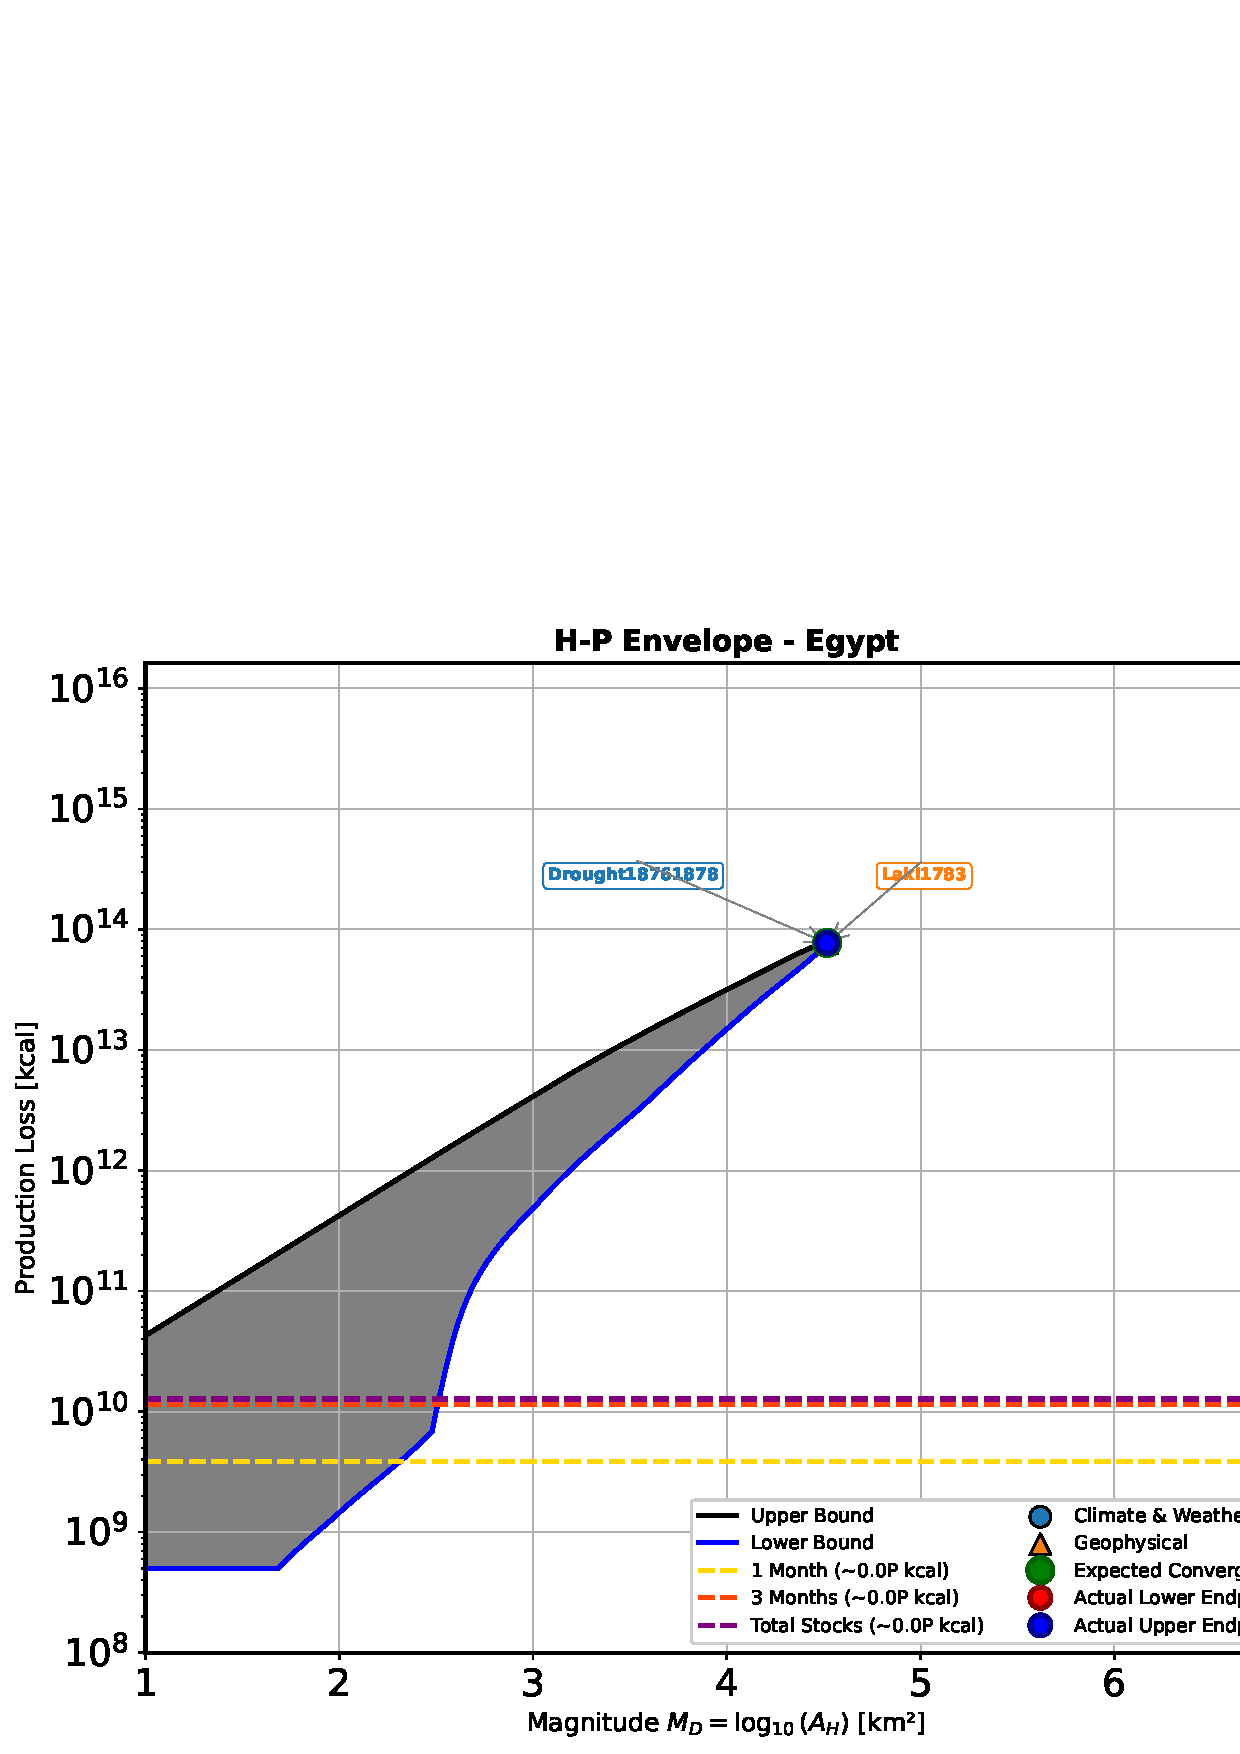
\includegraphics[width=\textwidth]{figure2_egypt_individual.png}
        \caption{Egypt (Concentrated Topology)}
    \end{subfigure}
    \hfill
    \begin{subfigure}[b]{0.48\textwidth}
        \centering
        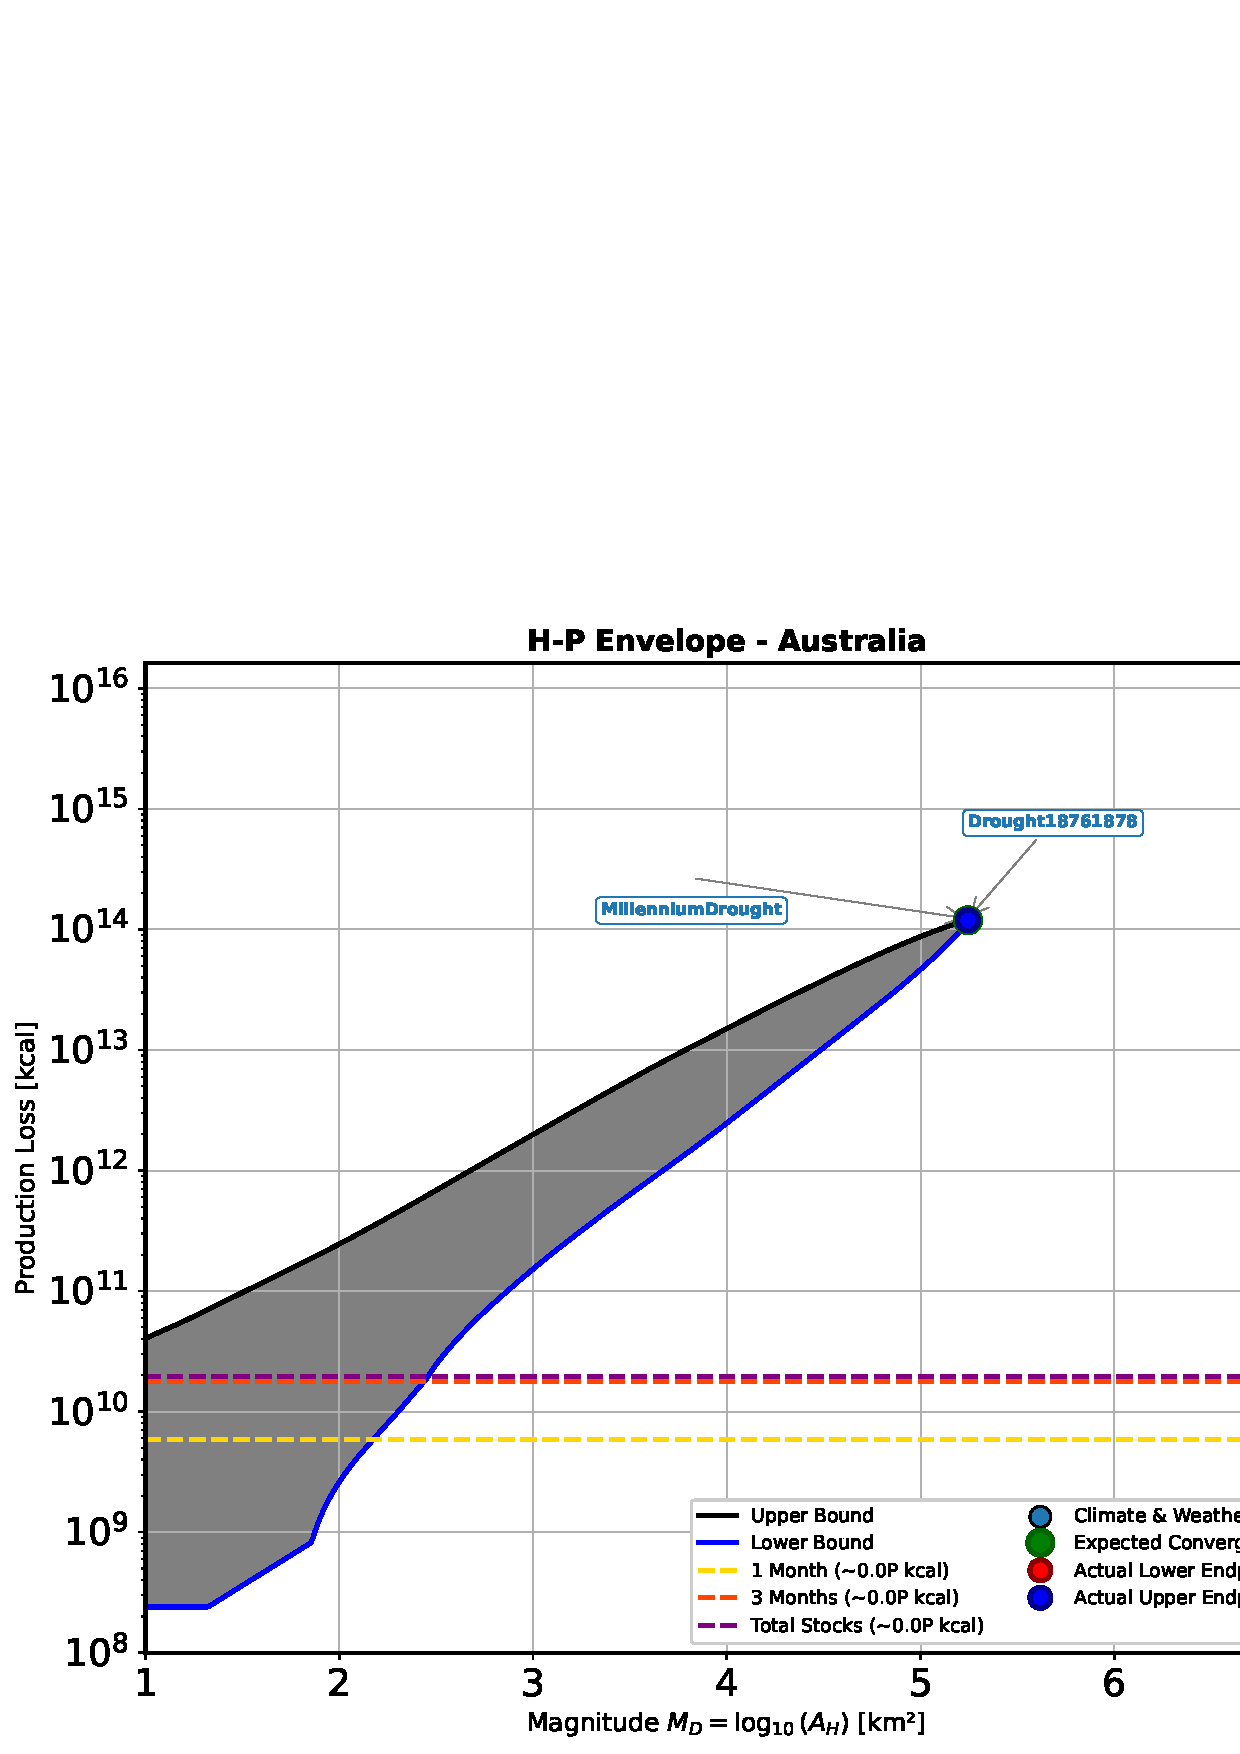
\includegraphics[width=\textwidth]{figure2_australia_individual.png}
        \caption{Australia (Export Topology)}
    \end{subfigure}
    \caption{\textbf{Additional National H-P Envelopes.} 
    (a) Egypt exhibits a highly "stiff" envelope due to the extreme concentration of agriculture in the Nile Delta, where small spatial extents ($M_D \approx 4$) correspond to massive production proportions. 
    (b) Australia shows a wider uncertainty band reflecting the geographic spread of its wheat belt. Dashed lines indicate national food security thresholds scaled from global stocks.}
    \label{fig:S2_additional_countries}
\end{figure}

\clearpage

\section*{Supplementary Tables}
\addcontentsline{toc}{section}{Supplementary Tables}

\begin{table}[H]
    \centering
    \caption{\textbf{National Food Security Thresholds.} 
    Verification values for the consumption-based thresholds used in Figure 2. Thresholds are calculated by scaling global USDA stocks-to-use ratios by each country's annual caloric production (derived from SPAM 2020). "Total Stocks" represents the theoretical systemic failure point if reserves were fully depleted.}
    \label{tab:S1_country_stocks}
    \vspace{0.2cm}
    \resizebox{\textwidth}{!}{%
    \begin{tabular}{lccccc}
        \toprule
        \textbf{Country} & \textbf{Annual Production} & \textbf{Harvest Area} & \textbf{1-Month Supply} & \textbf{3-Month Supply} & \textbf{Total Stocks} \\
         & (kcal) & (km$^2$) & (kcal) & (kcal) & (kcal) \\
        \midrule
        USA & $1.54 \times 10^{15}$ & 532,806 & $7.62 \times 10^{10}$ & $2.29 \times 10^{11}$ & $2.53 \times 10^{11}$ \\
        China & $2.19 \times 10^{15}$ & 985,311 & $1.08 \times 10^{11}$ & $3.25 \times 10^{11}$ & $3.60 \times 10^{11}$ \\
        India & $1.16 \times 10^{15}$ & 918,636 & $5.77 \times 10^{10}$ & $1.73 \times 10^{11}$ & $1.92 \times 10^{11}$ \\
        Brazil & $4.24 \times 10^{14}$ & 239,080 & $2.10 \times 10^{10}$ & $6.31 \times 10^{10}$ & $6.99 \times 10^{10}$ \\
        France & $2.19 \times 10^{14}$ & 92,084 & $1.09 \times 10^{10}$ & $3.26 \times 10^{10}$ & $3.61 \times 10^{10}$ \\
        Egypt & $7.72 \times 10^{13}$ & 32,950 & $3.83 \times 10^{09}$ & $1.15 \times 10^{10}$ & $1.27 \times 10^{10}$ \\
        Australia & $1.19 \times 10^{14}$ & 175,650 & $5.90 \times 10^{09}$ & $1.77 \times 10^{10}$ & $1.96 \times 10^{10}$ \\
        Argentina & $3.01 \times 10^{14}$ & 162,543 & $1.49 \times 10^{10}$ & $4.47 \times 10^{10}$ & $4.95 \times 10^{10}$ \\
        \bottomrule
    \end{tabular}
    }
\end{table}

\newpage

\section*{Supplementary References}
\addcontentsline{toc}{section}{Supplementary References}

\bibliographystyle{unsrt}  % Numbered style for Nature
\bibliography{references}

% If you want to manually enter references Nature style:
% \begin{enumerate}
% \item Yu, Q. et al. Spatial production allocation model (SPAM) 2010 v2.0. \textit{MapSPAM} (2020).
% \item You, L. et al. Spatial production allocation model (SPAM) 2005 version 3 release 2. \textit{IFPRI} (2014).
% \item Hanks, T. C. \& Kanamori, H. A moment magnitude scale. \textit{J. Geophys. Res.} \textbf{84}, 2348--2350 (1979).
% \item Lobell, D. B., Schlenker, W. \& Costa-Roberts, J. Climate trends and global crop production since 1980. \textit{Science} \textbf{333}, 616--620 (2011).
% \item Porter, J. R. et al. Food security and food production systems. \textit{Climate Change 2014: Impacts, Adaptation, and Vulnerability} 485--533 (2014).
% \item Cormen, T. H., Leiserson, C. E., Rivest, R. L. \& Stein, C. \textit{Introduction to Algorithms} 3rd edn (MIT Press, 2009).
% \item Dantzig, G. B. Discrete-variable extremum problems. \textit{Oper. Res.} \textbf{5}, 266--277 (1957).
% \item Beck, K. \textit{Test-Driven Development: By Example} (Addison-Wesley, 2003).
% \end{enumerate}

\end{document}
